\section{Hyperelastic materials}
Hyperelastiy is a special case of the classical elasticity brought to extreme conditions. At large strains they behave and in a nonlinear fashion in contrast to the linear stress-strain relation of the small strain elastic behavior. 
Other characteristics include the incompressibility which has direct consequences on the FEM it gives rise to volumetric locking which will be detailed in section 4.2. 
This kind of behavior is usually found in polymer characterized with a cross-linked network

\begin{figure}[h]
\centering
  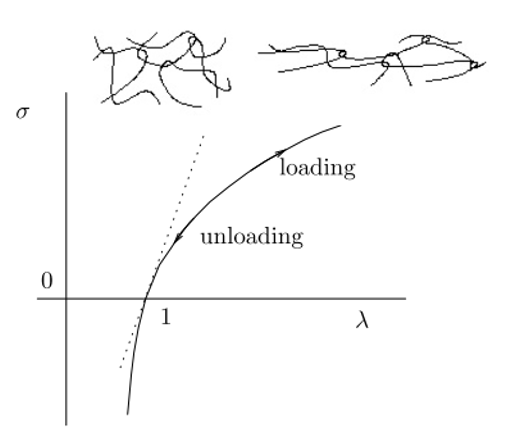
\includegraphics[height=5cm]{img/strainstress.PNG}
   \caption{Non-linear strain-stress curve with above a representation of a compressed an stretched polymer network.}
 \label{fgr:graft}
\end{figure}

The most outstanding property of elastomers is their ability
to undergo large deformations under relatively small stresses and
to retain initial configuration without considerable permanent
deformation after stress removal. This behavior is mostly governed
by changes of network entropy as the orientation of chains alters
with deformation. These basic features can be well described by statistical mechanics as done by Treolar. However, due to the development of computational mechanics and finite element analysis the invariant-based continuum mechanics theory is used to predict rubber elasticity.
\subsection{Constitutive Modeling}
Elastomers exhibit a complicated nonlinear behavior including
hysteresis, viscoelasticity and stress softening phenomenon. The
latter case called Mullins effect, occurs in first cycles of loading. Hysteresis and
viscoelastic behavior take place due to deviation from static
deformation, in which the effects of time and deformation rate
must be taken into account. In the case of static
deformations, rubbers exhibit hyperelastic behavior; Thus, a strain
energy density function, W, can be attributed.
Stress-strain behavior cannot be described by simple hookean law but need something more complex in this case a strain energy density function W. It represents the work that must be done on unit volume of the material in the reference (unstrained) state to deform it to the current configuration. Strictly, W is the Helmholtz free energy in an isothermal process.
For isotropic materials (e.g., rubbers), strain energy function
(SEF) can be represented in terms of right (or left) Cauchy-Green
tensor \textbf{C} (or \textbf{B}) invariants ($I_1, I_2, I_3$) or eigen values of deformation
gradient tensor F, called principal stretches ($\lambda_1, \lambda_2, \lambda_3$). i.e.,
\begin{equation}
W=W(I_1, I_2, I_3)\\
\end{equation}
Where
\begin{align*}
I_1&=\textrm{tr}(\textnormal{\textbf{C}})=\lambda_1^2+\lambda_2^2+\lambda_3^2&\\
I_2&=\frac{1}{2}\left[I^2_1-(\textnormal{\textbf{C}}^2)\right]=\lambda_1^2\lambda_2^2+\lambda_2^2\lambda_3^2+\lambda_1^2\lambda_3^2&\\
I_3&=\textrm{det}(\textnormal{\textbf{C}})=\lambda_1^2\lambda_2^2\lambda_3^2&
\end{align*}
tr and det demonstrate trace and determinant of a tensor. The form
of strain energy density function depends on symmetry, thermodynamic,
energetic and entropic considerations. For example, in the
case of rubber-like materials, due to the negligible compressibility
under conventional pressures, incompressibility assumption is
often used ($I_3 = 1$).

\begin{equation}
W_R=\sum_{i,j=0}^{\infty} C_{ij}(I_1-3)^i(I_2-3)^j
\end{equation}

If a compressibility term is added it gives the expression of the generalized Rivlin model, a general
If only the first term is maintained one obtains the Neo-Hookean model.

\begin{equation}
W_{NH}= C_{10}(I_1-3)
\end{equation}

While if keeping the second term gives rise to the Mooney-Rivlin model.
\begin{equation}
W_{MR}= C_{10}(I_1-3)+C_{01}(I_2-3)
\end{equation}
Working with the framework of the generalized Rivlin model, also called polynomial hyperelastic model, other scientists have come up withhigher order models  to better predict the deviation from the neo-Hooken behavior at large stretches. Among them are: Yeoh, Gent, Arruda \& Boyce.
Another model of high value is the Ogden model, based on a stretch continuum mechanics treatment.
\begin{equation}
W_{O}= \sum_n \frac{\mu_n}{\alpha_n}(\lambda_1^{\alpha_n}+\lambda_2^{\alpha_n}+\lambda_3^{\alpha_n}-3)
\end{equation}
where $\mu_n$ and $\alpha_n$ are real constants.
One approach consists in dividing the strain energy function into deviatoric strain and hydrostatic strain.
\begin{equation}
W=W_D(I_2,I_2)+W_H(J)
\end{equation}

\subsection{Software implementation}
Material curve fitting allows you to derive coefficients from experimental data that
you provide for your material.
• With this capability, you compare experimental data versus program-calculated data
for different nonlinear models and determine the best material model to use.
• ANSYS provides curve-fitting, based on experimental data, for all of the available
hyperelastic models. Any of the hyperelasticity models in ANSYS can be used.
ANSYS implements both a linear and a nonlinear least-squares fit procedures for fitting the data•The common test types include:
 –Uniaxial test –Equi/biaxialtest –Shear test (planar test) –Volumetric tes
 
 Depending on the model you choose, hyperelastic curve fitting can be a linear or a nonlinear regression process. In both cases, the initial coefficients you supply will determine how accurate and efficient your curve fit will be. The initial values of the coefficients generally come from experience, and also from studying the function that defines the model you are attempting to compare/fit your data to. For most hyperelastic models, 1 or -1 is a good starting point. However, coefficient values can vary greatly depending on the model chosen. The Gent model, for instance, provides good fit with initial coefficient values as high as 1000. 
 
 Your error norms can be either normalized or non-normalized. Normalized error norms (the default regression option) generally give better results than the non-normalized error norms, since normalized error gives equal weight to all of your data points.

The solution control parameters of a nonlinear regression include:

    Number of iterations

    Residual tolerance

    Coefficient change tolerance

The solution stops when both the residual tolerance and the coefficient change tolerance of your error norm are met, or if the number of iterations criteria is met. When you use nonlinear regression, you must initialize your coefficients. 

The two factors you consider in determining results acceptability are visual fit and the error norm/residual values. When you plot the curve, the error norm/residual values are printed in the curve-fitting GUI window. Error norm values help you determine the quality of curve fitting and whether to accept the results, but are not always the best indicator of a valid curve fit. Plotting the curves and visually assessing the result is usually the best indication.
\subsubsection{Curve Fitting Problem}
Curve Fitting aims to fit one or more parameters of a model equation $\sigma ( \lambda$, Parameters) in such a way that a given curve $\sigma_M(\lambda)$ is approximated as closely as possible. In this
study, the stress-strain curve for simple shear and the combined stress-stretch curve for
tension and compression have to be approximated. The stress-stretch curve in tension
and compression will be used to explain the regression analysis process. The process for
simple shear is analogous.
Ideally, the fitted model equation resulting from regression analysis should yield the
same stress values as the measured curve.
\begin{equation}
\sigma(\lambda, \textnormal{Parameters})=\sigma_M(\lambda)
\end{equation}

Where $\sigma ( \lambda$, Parameters) is the model function, which depends on stretch and parameters,
and $\sigma_M(\lambda)$ denotes the measured stress-stretch curve.
The model equation for compression and tension is
\begin{equation}
\sigma=f(\lambda, C_{10}, C_{01}, C_{20}, C_{02}, C_{11})
\end{equation}

The parameters (material constants) $C_{ij}$ are considered constant and have to be determined
through regression analysis. Furthermore, in the compression/tension model
equation, they only appear linearly. As the number of data pairs within the measured
stress-stretch curve greatly exceeds the number of parameters within the model equation,
the problem definition is to solve an overdetermined system of linear equations
(Hartmann 2001) in such a way that a satisfactory goodness of fit is achieved.

\subsubsection{Regression analysis}
In general, the overdetermined system of linear equations from subsection 2.2 cannot be
solved. In order to overcome this problem, regression analysis can be applied. A set of
parameters, which yields to a curve that is as close to the measured curve as possible, has
to be determined. For a satisfactory curve fit, the difference between the stress values of
the measured curve and the model equation has to be small for a wide rage of stretches.
The least squares method uses the sum of the difference of the ordinates of two stress
values as an error criterion (Papula 2008, p. 691), which has to be minimized:
\begin{equation}
\epsilon_{ls}=\sum^n_{i=1}\left(\sigma_M(\lambda_i)-\sigma(\lambda_i, C_{10}, C_{01}, C_{20}, C_{02}, C_{11})\right)^2 
\end{equation}
Where $\epsilon_{ls}$: Least square error, $i$: Number of measured data pairs, $\lambda_i$: Measured stretch value, $\sigma_M(\lambda_i$: Measured stress at $\lambda_i$, $\sigma(\lambda_i, C_{10}, C_{01}, C_{20}, C_{02}, C_{11})$: Computed stress value of the model function at $\lambda_i$.
In ANSYS1, the above equation is called “unnormalized least squares fit” ANSYS Inc. (August
2002).
Since it is biased towards higher stress values, a weighted error criterion is
more useful in many cases. Equation 32 accounts equally for every stress value and is
called “normalized least square fit” ANSYS Inc. (August 2002).
\begin{equation}
\epsilon_{norm}=\sum^n_{i=1}\left(1- \frac{\sigma(\lambda_i, C_{10}, C_{01}, C_{20}, C_{02}, C_{11})}{\sigma_M(\lambda_i)}\right)^2 
\end{equation}

Note that Equation 32 would lead to a division by zero if $\sigma_M(\lambda_i)=0$. For this case
an exception has to be added. 
The software ANSYS offers a curve fitting module for hyperelastic material models.2
However, despite supporting higher order constitutive equations for input of material
constants, not all supported material models can be fitted up to these orders. Hence,
the Equations 20 and 28 and both error criteria3 were implemented in a Scilab4 script in
order to be able to fit higher order constitutive equations. The minimization algorithm
used in Scilab is Nelder-Mead (Nelder \& Mead 1965).

Curve fitting algorithm
The material constants are determined by a least-squares procedure for a given set of experimental data, which minimizes the relative error, solution.
The Mooney, Polynomial, Yeoh strain energy potentials are linear in terms of the constants. Therefore a linear least-square fit procedure is used.
The Ogden, Arruda-Boyce , Gent strain energy potentials are nonlinear in terms of the constants. A nonlinear least-squares fitting procedure is neede. We use Marquard-Levenberg algorithm.

\subsection{Numerical issues}
\subsubsection{Incompressibility and Volumetric Locking}
The Poisson ratio ($\nu$) of an isotropic material is usually defined as the ratio, taken with the
opposite sign, between its lateral and longitudinal strains under the action of longitudinal
stresses. 
Some materials exhibit isochoric deformation. This means that the volume of the body stays constant and thus $\nu = 0.5$. If displacement based low-order continuum elements are used this situation cannot be properly simulated. Such elements behave excessively stiff and are said to undergo volumetric locking. Fully integrated and linear brick elements suffer from this issue.  The trivial solution is to use higher order elements. As such, these have higher degrees of freedom so even if incompressible, the strain can still be variable in the element. Higher order elements solve the problem, but are computationally costly. A cheaper solution is using under integrated elements. As only one integration point is available in the center, strain is constant but locking does not occur, however higher mesh density will be necessary.  Another solution is to separate volumetric strain $\epsilon_v$ from deviatoric strain $\epsilon_d$. THe former are integrated in the center and the latter using the full
Although they are considered incompressible they are actually only nearly incompressible. This aspect can be integrated into FEM for complex deformation to help avoid numerical problems that can arise due to incompressible formulations. 
The term $\sum^N_{k=1}\frac{1}{d_k}(J-1)^{2k}$ where $d_k$ is the incompressibility parameter
\subsubsection{Mixed formulation}
\subsubsection{Reduced integration}

\subsubsection{Shear locking}
Full and reduced integration 
\paragraph{Mixed Formulation}
\subsubsection{Hourglassing}

